\documentclass{article}

\usepackage{amsfonts}
\usepackage{pdfpages}
\usepackage[margin=1in]{geometry}

\title{ STAT 321: Assignment 3}
\author{Saksham Sudershan}
\date{19 February 2022}

\begin{document}
	\maketitle
	\section*{Problem 1}
		\subsection*{(a)}
			$$ \mathbb{E}(N|R=r) = n \times p \; \; \; \; \; \; \; \; \; where\ p\ is\ the\ probability\ of\ success $$
			$$ \mathbb{E}(N|R=r) = 10 \times \frac{r}{10}  $$
			$$ \mathbb{E}(N|R=r) = r $$
		\subsection*{(b)}
			$$ \mathbb{V}ar[N|R=r] =  n \times p \times (1-p) $$
			$$ \mathbb{V}ar[N|R=r] = 10 \times \frac{r}{10} \times \left(1-\frac{r}{10}\right)  $$
			$$ \mathbb{V}ar[N|R=r] = r \times \left(1-\frac{r}{10}\right)  $$
		\subsection*{(c)}
			$$ \mathbb{E}(R) = \frac{1+2+3+4+5+6+7+8+9+10}{10}=\frac{55}{10} $$
			$$ \mathbb{E}(R) = 5.5 = r $$
			$$ \mathbb{E}(N) = r $$

			$$ \mathbb{E}(N) = 5.5 $$
		\subsection*{(d)}
			Using the Law of Total Variance,
			$$ \mathbb{V}ar(N) = \mathbb{E}\left[\mathbb{V}ar(N|R)\right] + \mathbb{V}ar\left(\mathbb{E}[N|R]\right) $$
			$$ = \mathbb{E}\left[ r \times \left(1-\frac{r}{10}\right) \right] + \mathbb{V}ar(r)$$

			We know that $\mathbb{E}[r] = \bar r =  5.5$. Now $\mathbb{V}ar(r)$ is given by,
			$$ \mathbb{V}ar(r) = \frac{\sum_{i=1}^{10}(r_i - \bar{r})^2}{10} $$
			$$ \mathbb{V}ar(r) = (1-5.5)^2 + (2-5.5)^2 +(3-5.5)^2+(4-5.5)^2+(5-5.5)^2 $$
			$$ \frac{+(6-5.5)^2+(7-5.5)^2+(8-5.5)^2+(9-5.5)^2+(10-5.5)^2}{10} $$
			$$ \mathbb{V}ar(r) = \frac{82.5}{10} = 8.25 $$
			
			And $ \mathbb{E}\left[ r \times \left(1-\frac{r}{10}\right) \right]$ is given by,
			$$ \mathbb{E}(r) - \frac{1}{10} \times \mathbb{E}(r^2) = 5.5 - \frac{1}{10} \times 38.5 $$

			So,
			$$ \mathbb{V}ar(N) =5.5-3.85 + 8.25 $$
			$$ \Rightarrow \mathbb{V}ar(N) = 9.9 $$
	
	\section*{Problem 2}
		\subsection*{(a)}
			The discrete probability mass function $p(x_1,x_2)$ is given by,
			\begin{center}
			\begin{tabular}{ |c|c|c|c|c|}
			\hline
			& & & &  \\
			$\frac{X_1=}{X_2=}$ & 0 & 1 & 2 & 3 \\
			& & & &  \\
			\hline
			& & & &  \\
			0 & $\frac{{3 \choose 3}}{{14 \choose 3}}$ & $\frac{{5 \choose 1}\times{3 \choose 2}}{{14 \choose 3}}$ & $\frac{{5 \choose 2}\times{3 \choose 1}}{{14 \choose 3}}$ & $\frac{{5 \choose 3}}{{14 \choose 3}}$  \\
			& & & &  \\
			\hline
			& & & &  \\
			1 & $\frac{{6 \choose 1}\times{3 \choose 2}}{{14 \choose 3}}$  & $\frac{{5 \choose 1}\times{6 \choose 1}\times{3 \choose 1}}{{14 \choose 3}}$ & $\frac{{5 \choose 2}\times{6 \choose 1}}{{14 \choose 3}}$ & 0  \\
			& & & &  \\
			\hline
			& & & &  \\
			2 & $\frac{{6 \choose 2}\times{3 \choose 1}}{{14 \choose 3}}$ & $\frac{{6 \choose 2}\times{5 \choose 1}}{{14 \choose 3}}$ & 0 & 0 \\
			& & & &  \\
			\hline
			& & & &  \\
			3 & $\frac{{6 \choose 3}}{{14 \choose 3}}$ & 0 & 0 & 0 \\
			& & & &  \\
			\hline
			\end{tabular}
			\end{center}

			This can be further simplified to,
			\begin{center}
			\begin{tabular}{ |c|c|c|c|c|}
			\hline
			& & & &  \\
			$\frac{X_1=}{X_2=}$ & 0 & 1 & 2 & 3 \\
			& & & &  \\
			\hline
			& & & &  \\
			0 & $\frac{1}{364}$ & $\frac{15}{364}$ & $\frac{30}{364}$ & $\frac{10}{364}$  \\
			& & & &  \\
			\hline
			& & & &  \\
			1 & $\frac{18}{364}$  & $\frac{90}{364}$ & $\frac{60}{364}$ & 0  \\
			& & & &  \\
			\hline
			& & & &  \\
			2 & $\frac{45}{364}$ & $\frac{75}{364}$ & 0 & 0 \\
			& & & &  \\
			\hline
			& & & &  \\
			3 & $\frac{20}{364}$ & 0 & 0 & 0 \\
			& & & &  \\
			\hline
			\end{tabular}
			\end{center}
		\subsection*{(b)}
			The marginal probability mass function $p(x_1)$ is given by,
			\begin{center}
			\begin{tabular}{|c|c|c|c|c|}
			\hline
			$X_1=$ & 0 & 1 & 2 & 3 \\
			\hline
			& & & & \\
			& $\frac{84}{364}$ & $\frac{180}{364}$ & $\frac{90}{364}$ & $\frac{10}{364}$ \\ 
			& & & & \\
			\hline
			\end{tabular}
			\end{center}
			
			And the marginal probability mass function $p(x_2)$ is given by,
			\begin{center}
			\begin{tabular}{|c|c|c|c|c|}
			\hline
			$X_2=$ & 0 & 1 & 2 & 3 \\
			\hline
			& & & & \\
			& $\frac{56}{364}$ & $\frac{168}{364}$ & $\frac{120}{364}$ & $\frac{20}{364}$ \\ 
			& & & & \\
			\hline
			\end{tabular}
			\end{center}

		\subsection*{(c)}
			To calculate the correlation between $X_1$ and $X_2$, we can first calculate the covariance,
			$$ Cov(X_1,X_2) = \sum_{(x,y) \in S} (x_1-\mu_{x_1})(x_2-\mu_{x_2})f(x_1,x_2) $$
			From the marginal probability mass function, we know that $\mu_{x_1}=1.07$ and $\mu_{x_2}=1.28$.
			$$ \Rightarrow Cov(X_1,X_2) = (0-1.0714)(0-1.2857)\left(\frac{1}{364}\right)+(1-1.0714)(0-1.2857)\left(\frac{15}{364}\right)+(2-1.0714)(0-1.2857)\left(\frac{30}{364}\right)$$
			$$ +(3-1.0714)(0-1.2857)\left(\frac{10}{364}\right)+(0-1.0714)(1-1.2857)\left(\frac{18}{364}\right)+(1-1.0714)(1-1.2857)\left(\frac{90}{364}\right)$$
			$$ +(2-1.0714)(1-1.2857\left(\frac{60}{364}\right)+(0-1.0714)(2-1.2857)\left(\frac{45}{364}\right)+(1-1.0714)(2-1.2857)\left(\frac{75}{364}\right)$$
			$$ +(0-1.0714)(3-1.2857)\left(\frac{20}{364}\right) $$

			$$ \Rightarrow Cov(X_1,X_2) \approx -0.388 $$

			We also have to find the standard deviations of $X_1$ and $X_2$,
			$$ \sigma_{X_1} = \sum_{i=1}^4 (x_{1_i} - \mu_{x_1}) = \sqrt{\frac{1458}{2548}} $$
			$$ and\ \sigma_{X_2} = \sum_{i=1}^4 (x_{2_i} - \mu_{x_2}) = \sqrt{\frac{396}{637}} $$

			$$ Therefore\ Corr(X_1,X_2) \approx \frac{-0.388}{0.596} = -0.651 $$
	
	\section*{Problem 3}
		\subsection*{(a)}
			We can find $c$ by equating the total probability equal to 1. So,
			$$ \int_0^{30} c(6-t)^2 dt = 1 $$
			$$ \Rightarrow c \int_0^{30} (6-t)^2 dt = 1 $$
			$$ \Rightarrow c \int_0^{30} 36+t^2-12t dt = 1 $$
			$$ \Rightarrow c \left[ 36t +\frac{t^3}{3} -6t^2 \right]_0^{30} = 1 $$
			$$ \Rightarrow c \times 4680 = 1 $$
			$$ \Rightarrow c = \frac{1}{4680} $$

		\subsection*{(b)}
			The cumulative distribution function is given by,
			$$ F(t) = P(T \leq t) $$
			$$ \int_0^{t} f(t) dt = \frac{1}{4680} \int_0^{t}  (6-t)^2  dt$$
			$$ = \frac{1}{4680} \left[ 36t+ \frac{t^3}{3} -6 t^2 \right]_0^t $$
			$$ = \frac{1}{4680} \left[ 36t+ \frac{t^3}{3} -6 t^2 \right] $$

			$$ \Rightarrow F(t) = 0, when\ t < 0 $$
			$$ and\ F(t) =  \frac{1}{4680} \left[ 36t+ \frac{t^3}{3} -6 t^2 \right], when\ 0 \leq t \leq 30 $$
			$$ and\ F(t) = 1, when\ t > 30 $$

		\subsection*{(c)}
			The probability that a student will wait more than 10 minutes is given by,
			$$ P(T > 10) = 1 - P( T \leq 10) $$
			$$ = 1 - F(10) $$
			$$ = 1 - \frac{1}{4680} \left[ 36t+ \frac{t^3}{3} -6 t^2 \right] $$
			$$ \Rightarrow P(T>10) \approx 0.9801 $$

		\subsection*{(d)}
			The probability that a student will wait more than 20 minutes given that they have waited for 10 minutes is given by,
			$$ P(T \geq 20 | T>10) = \frac{P(T \geq 20 \cap T > 10)}{P(T>10)} $$

			Similar to the previous question, this can be written as,
			$$ \frac{1-F(20)}{1-F(10)} = \frac{277/351}{344/351} = 0.80523 $$

		\subsection*{(e)}
			The probability that a student will be late for class is given by,
			$$ P(T>20) = 1-F(20) $$
			$$ \Rightarrow P(T>20) = \frac{277}{351} = 0.789 $$

			Using the binomial distribution, setting the probability of being late as the probability of success, $p=0.789$.
			Then,
			$$ P(3\ students\ are\ late) = {n \choose r} (p)^r (1-p)^{n-r} = {10 \choose 3} (0.789)^3 (1-0.789)^7 $$
			$$ So,\ P(3\ students\ are\ late) \approx 0.0011 $$

	\section*{Problem 4}
		\subsection*{(a)}
			We know that $Y \sim exp(\lambda)$. So, the probability distribution function of Y is given by,
			$$ f_y(y) = \lambda e^{-\lambda y} $$
			And the cumulative distribution function of Y is given by,
			$$ F_y(y) = 1-e^{-\lambda y} = P(Y \leq y) $$
			
			And $X = \lfloor Y \rfloor + 1$. So, the probability distribution function of $X$ is given by,
			$$ f_x(x) = P(X=x) $$
			We know that $X$ takes the value $k$, whenever $k-1 \leq Y \leq k$, so
			$$ f_x(x) = P(x-1\leq Y \leq x) $$
			Thus, we are trying to find the probability that Y lies between $x$ and $x-1$. This can also be written as,
			$$ P(Y \leq x) - P(Y \leq k-1) $$
			$$ = F_y(k) - F_y(k-1) $$
			Using the cdf of Y, this can be written as
			$$ \left( 1-e^{-\lambda x} \right) - \left( 1 - e^{-\lambda (x-1)} \right) $$
			$$ = 1 -e^{-\lambda x}-1+-e^{-\lambda (x-1)} $$
			$$ =e^{-\lambda (x-1)}-e^{-\lambda x}$$
			$$ = e^{-\lambda x} \cdot e^{\lambda} -e^{-\lambda x} $$
			$$ = e^{-\lambda x}[e^\lambda -1] $$
			Now, multiplying and dividing by $e^\lambda$, this becomes
			$$ = e^{-\lambda x} \cdot e^{\lambda} \left[\frac{e^\lambda}{e^\lambda}-\frac{1}{e^\lambda}\right]$$
			$$ \Rightarrow f_x(x)= e^{-\lambda (x-1)} [1-e^{-\lambda}]$$ 

			This resembles the probability distribution function of a geometric distribution, where the probability of success is given by $1-e^{-\lambda}$. So we can say that,
			$$ X \sim Geom(p) \; \; \; \; \; \; \; \; ,where\ p = 1-e^{-\lambda}$$

	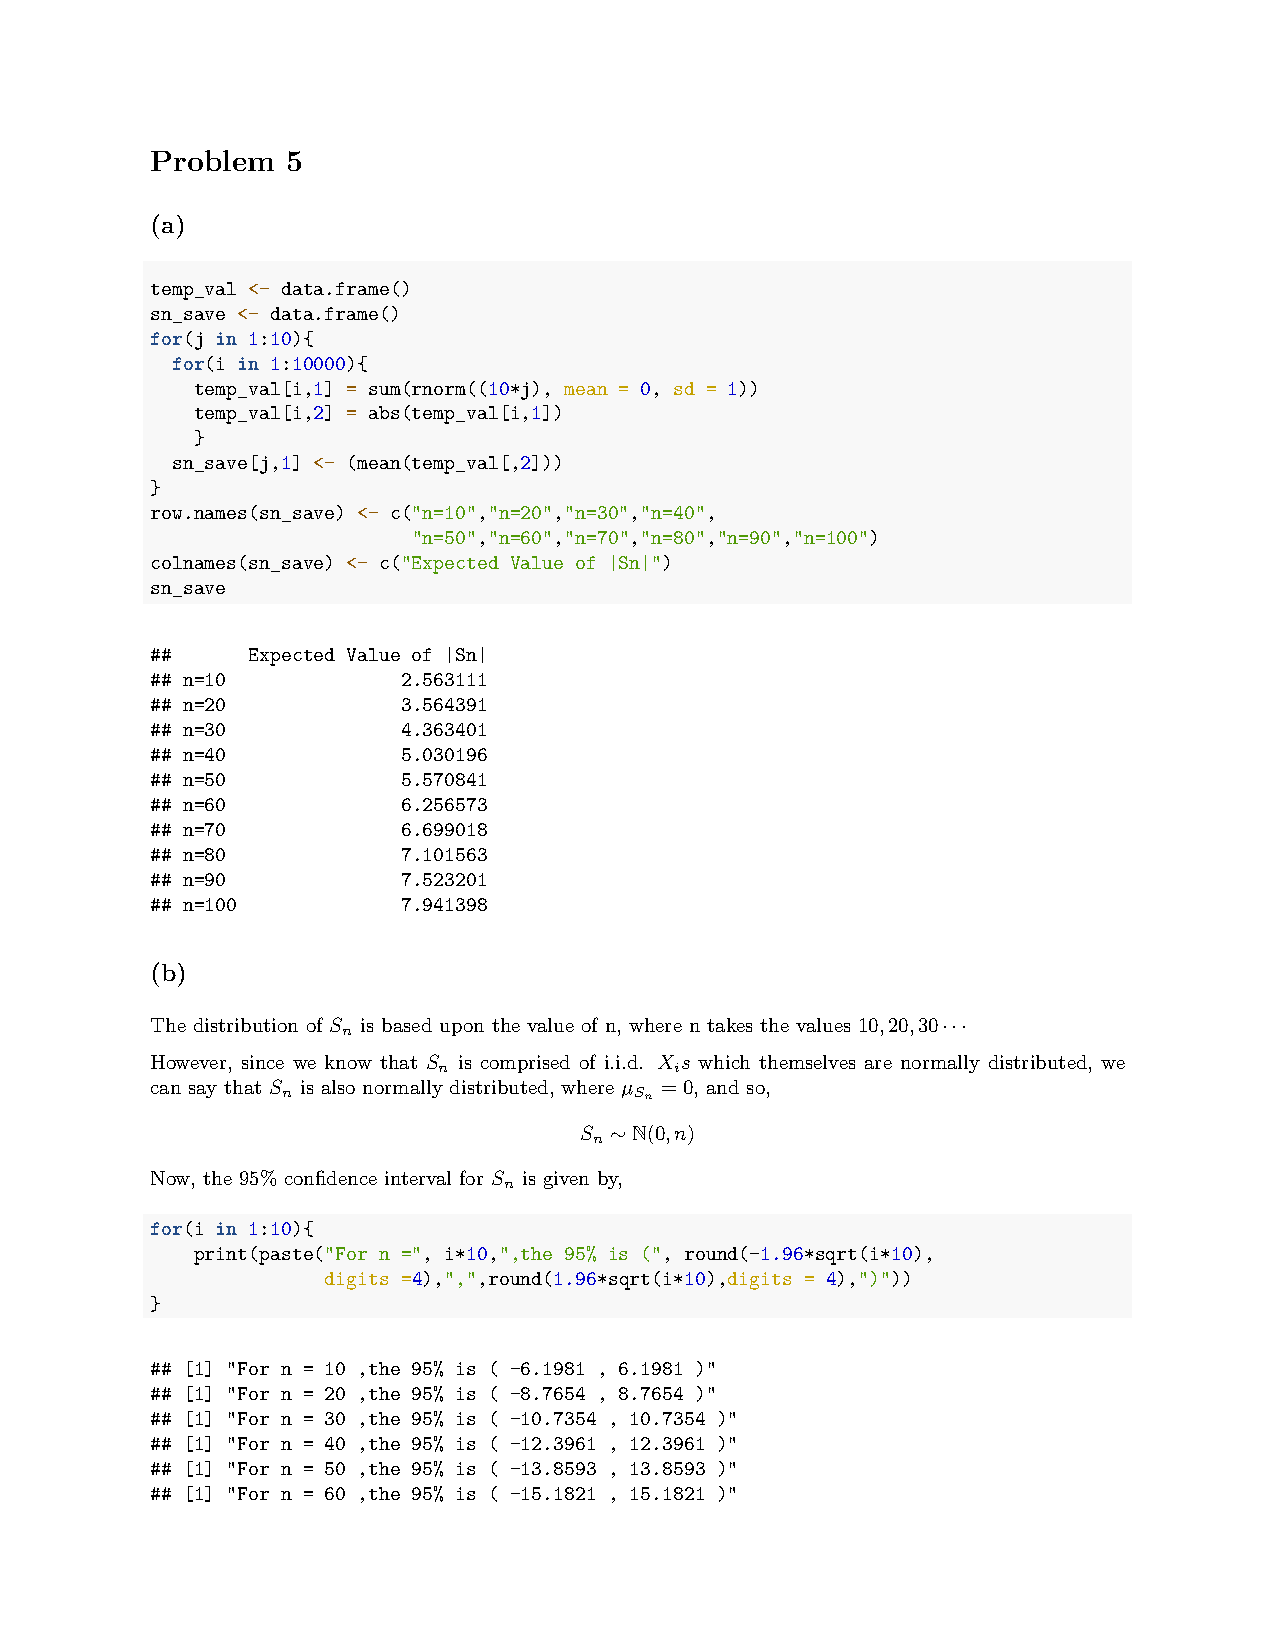
\includepdf[pages=-, pagecommand={}]{Ass3-Part1.pdf}
\end{document}